\documentclass[a4paper]{article}
\usepackage[margin=3cm]{geometry}
\usepackage{graphicx}

\usepackage{hyperref}
\hypersetup{
	colorlinks=true,
	linkcolor=blue,
	filecolor=magenta,
	urlcolor=cyan,
	hyperindex=true,
	linktocpage=true,%makes the page number be the link in the index
}
\usepackage{listings}
\lstset{
	basicstyle=\tiny\ttfamily,
	columns=fullflexible,
	keepspaces=true,
	breaklines=true,
	frame=single,
	showstringspaces=true,
	tabsize=4,
	showspaces=true,
	showtabs=true,
}
\usepackage{pgfplots}

\renewcommand{\arraystretch}{1.2}

\title{Exponential growth forecast of AI model size}

\author{Chaya2766}

\date{last updated \today}

\begin{document}
	\sffamily
	\hyphenchar\font=-1
	\sloppy
	
	\maketitle
	
	\textbf{
		\sloppy
		\hyphenchar\font=-1
		}
	
	\vfill
	
	\begin{abstract}
		Abstract goes here
	\end{abstract}
	
	\vfill
	
	\begin{quote}
		\begin{center}
			\textbf{DISCLAIMER AND WARNING}
		\end{center}
		
		This is not a scientific paper or engineering advice.
		This document is only intended as creative world‑building and has not been peer‑reviewed or approved for any practical application.
		Use of these ideas in real‑world designs or other serious application is entirely at the reader’s discretion and risk.
	\end{quote}
	
	%\noindent \rule{\linewidth}{1pt}
	\vfill
	
	\tableofcontents
	
	\pagebreak
	
	\section{Background and initial data}
	
	In the current AI craze, the size of AI models is growing very rapidly, and blindly extrapolating exponential growth from current data is not desired.
	
	I am instead making an assumption that the amount of resources that can be poured into AI training is limited by the total amount of resources available, and as such follows the same growth rate as the total GDP of humanity.
	
	\medskip
	
	In my previous document "humanity of the third millenium under assumption of exponential growth" I modeled the total global GDP of humanity as well as other data using simple exponential growth, and found that an annual growth rate of \textbf{2.88\%} fits the data best.
	
	\medskip
	
	The first AI model to be trained with \textbf{1 trillion parameters} that I am aware of was Kimi K2, released in \textbf{2025}.
	By necessity of how I model growth, I have to assume that after that point the growth of AI model size slowed drastically and matched the GDP growth.
	
	\bigskip
	
	The starting point is 2025, as such exponential function is set as:
	
	$$ 1E+15 \cdot 1.0288^{(x-2025)} $$
	
	\bigskip
	
	Keep in mind that this is not a prediction that AI model size will grow as described, but rather just a calculation of values and dates of milestones based on that assumption.
	
	\pagebreak
	
	\section{charts and data tables (years 2025 to 3000)}
	
	Horizontal lines and bold text mark the milestones of trillion, quadrillion, quintillion, sextillion and septillion parameters.
	
	\begin{center}
		linear scale
		
		\medskip
		
		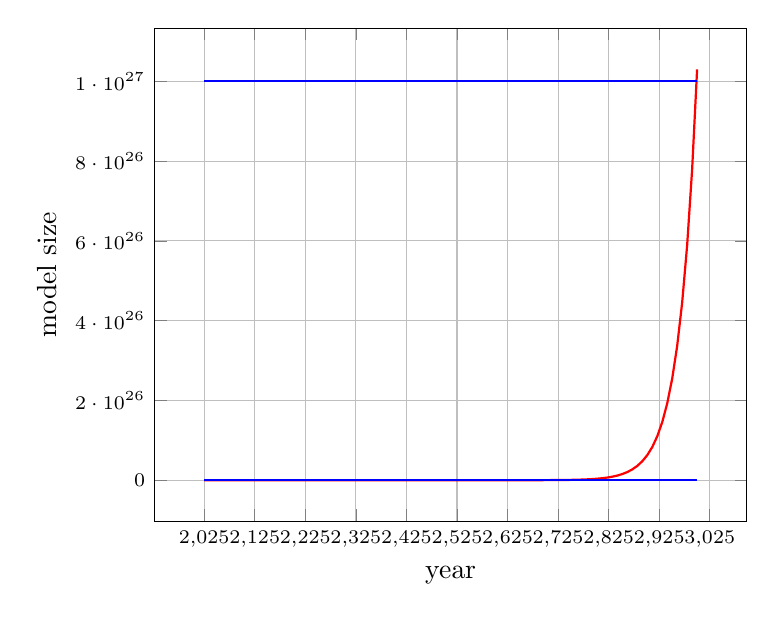
\begin{tikzpicture}
			\begin{axis}[
				width=0.75\linewidth,
				xlabel=year,
				ylabel=model size,
				scaled ticks=false,%disables scientific notation
				%ytick={0,10000,...},%forces every multiple of 10 000 to be shown
				xtick={2025,2125,...,3000},
				yticklabel style={font=\scriptsize},%makes axis numbers tiny
				xticklabel style={font=\scriptsize},%makes axis numbers tiny
				%ymode=log,
				%xmin=1, xmax=100,
				%ymin=0, ymax=10,
				grid=both,
				minor grid style={gray!25},
				major grid style={gray!50},
				]
				\addplot[red, thick, domain=2025:3000, samples=100]
				{1E+15 * pow(1.0288,x-2025)};
				\addplot[blue, thick, domain=2025:3000, samples=100]
				{1E+15};
				\addplot[blue, thick, domain=2025:3000, samples=100]
				{1E+18};
				\addplot[blue, thick, domain=2025:3000, samples=100]
				{1E+21};
				\addplot[blue, thick, domain=2025:3000, samples=100]
				{1E+24};
				\addplot[blue, thick, domain=2025:3000, samples=100]
				{1E+27};
			\end{axis}
		\end{tikzpicture}
		
		\medskip
		
		logarithmic scale
		
		\medskip
		
		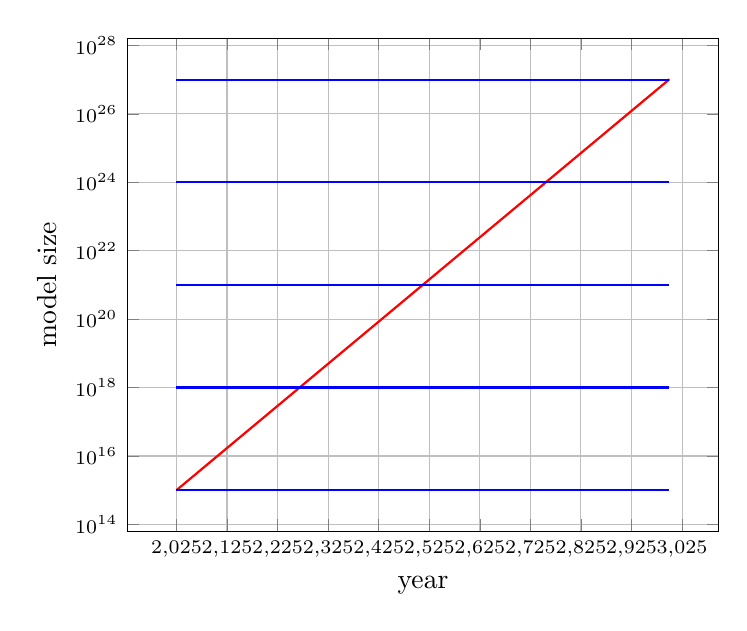
\begin{tikzpicture}
			\begin{axis}[
				width=0.75\linewidth,
				xlabel=year,
				ylabel=model size,
				scaled ticks=false,%disables scientific notation
				%ytick={0,10000,...},%forces every multiple of 10 000 to be shown
				xtick={2025,2125,...,3000},
				yticklabel style={font=\scriptsize},%makes axis numbers tiny
				xticklabel style={font=\scriptsize},%makes axis numbers tiny
				ymode=log,
				%xmin=1, xmax=100,
				%ymin=0, ymax=10,
				grid=both,
				minor grid style={gray!25},
				major grid style={gray!50},
				]
				\addplot[red, thick, domain=2025:3000, samples=100]
				{1E+15 * pow(1.0288,x-2025)};
				\addplot[blue, thick, domain=2025:3000, samples=100]
				{1E+15};
				\addplot[blue, thick, domain=2025:3000, samples=100]
				{1E+18};
				\addplot[blue, thick, domain=2025:3000, samples=100]
				{1E+21};
				\addplot[blue, thick, domain=2025:3000, samples=100]
				{1E+24};
				\addplot[blue, thick, domain=2025:3000, samples=100]
				{1E+27};
			\end{axis}
		\end{tikzpicture}
	\end{center}
	
	\pagebreak
	
	\small

    \begin{tabular}{| c | c |}
    	\hline
    	year & model size \\\hline
    	\textbf{2025} & \textbf{1.0000E+15} \\\hline
    	2030 & 1.1525E+15 \\\hline
    	2035 & 1.3283E+15 \\\hline
    	2040 & 1.5310E+15 \\\hline
    	2045 & 1.7645E+15 \\\hline
    	2050 & 2.0336E+15 \\\hline
    	2055 & 2.3438E+15 \\\hline
    	2060 & 2.7014E+15 \\\hline
    	2065 & 3.1134E+15 \\\hline
    	2070 & 3.5883E+15 \\\hline
    	2075 & 4.1357E+15 \\\hline
    	2080 & 4.7665E+15 \\\hline
    	2085 & 5.4936E+15 \\\hline
    	2090 & 6.3316E+15 \\\hline
    	2095 & 7.2974E+15 \\\hline
    	2100 & 8.4105E+15 \\\hline
    	2105 & 9.6934E+15 \\\hline
    	2110 & 1.1172E+16 \\\hline
    	2115 & 1.2876E+16 \\\hline
    	2120 & 1.4840E+16 \\\hline
    	2125 & 1.7104E+16 \\\hline
    	2130 & 1.9713E+16 \\\hline
    	2135 & 2.2720E+16 \\\hline
    	2140 & 2.6185E+16 \\\hline
    	2145 & 3.0180E+16 \\\hline
    	2150 & 3.4783E+16 \\\hline
    	2155 & 4.0089E+16 \\\hline
    	2160 & 4.6204E+16 \\\hline
    	2165 & 5.3252E+16 \\\hline
    	2170 & 6.1375E+16 \\\hline
    	2175 & 7.0736E+16 \\\hline
    	2180 & 8.1526E+16 \\\hline
    	2185 & 9.3962E+16 \\\hline
    	2190 & 1.0829E+17 \\\hline
    	2195 & 1.2481E+17 \\\hline
    	2200 & 1.4385E+17 \\\hline
    	2205 & 1.6580E+17 \\\hline
    	2210 & 1.9109E+17 \\\hline
    	2215 & 2.2023E+17 \\\hline
    	2220 & 2.5383E+17 \\\hline
    	2225 & 2.9254E+17 \\\hline
    	2230 & 3.3717E+17 \\\hline
    	2235 & 3.8860E+17 \\\hline
    	2240 & 4.4787E+17 \\\hline
    	2245 & 5.1619E+17 \\\hline
    	2250 & 5.9493E+17 \\\hline
    	2255 & 6.8568E+17 \\\hline
    	2260 & 7.9027E+17 \\\hline
    	2265 & 9.1081E+17 \\\hline
    \end{tabular}
    \hfill
    \begin{tabular}{| c | c |}
    	\hline
    	year & model size \\\hline
    	\textbf{2270} & \textbf{1.0497E+18} \\\hline
    	2275 & 1.2099E+18 \\\hline
    	2280 & 1.3944E+18 \\\hline
    	2285 & 1.6071E+18 \\\hline
    	2290 & 1.8523E+18 \\\hline
    	2295 & 2.1348E+18 \\\hline
    	2300 & 2.4604E+18 \\\hline
    	2305 & 2.8357E+18 \\\hline
    	2310 & 3.2683E+18 \\\hline
    	2315 & 3.7668E+18 \\\hline
    	2320 & 4.3414E+18 \\\hline
    	2325 & 5.0036E+18 \\\hline
    	2330 & 5.7669E+18 \\\hline
    	2335 & 6.6465E+18 \\\hline
    	2340 & 7.6604E+18 \\\hline
    	2345 & 8.8289E+18 \\\hline
    	2350 & 1.0176E+19 \\\hline
    	2355 & 1.1728E+19 \\\hline
    	2360 & 1.3517E+19 \\\hline
    	2365 & 1.5578E+19 \\\hline
    	2370 & 1.7955E+19 \\\hline
    	2375 & 2.0694E+19 \\\hline
    	2380 & 2.3850E+19 \\\hline
    	2385 & 2.7488E+19 \\\hline
    	2390 & 3.1681E+19 \\\hline
    	2395 & 3.6514E+19 \\\hline
    	2400 & 4.2083E+19 \\\hline
    	2405 & 4.8502E+19 \\\hline
    	2410 & 5.5901E+19 \\\hline
    	2415 & 6.4428E+19 \\\hline
    	2420 & 7.4255E+19 \\\hline
    	2425 & 8.5582E+19 \\\hline
    	2430 & 9.8636E+19 \\\hline
    	2435 & 1.1368E+20 \\\hline
    	2440 & 1.3102E+20 \\\hline
    	2445 & 1.5101E+20 \\\hline
    	2450 & 1.7404E+20 \\\hline
    	2455 & 2.0059E+20 \\\hline
    	2460 & 2.3119E+20 \\\hline
    	2465 & 2.6645E+20 \\\hline
    	2470 & 3.0710E+20 \\\hline
    	2475 & 3.5394E+20 \\\hline
    	2480 & 4.0793E+20 \\\hline
    	2485 & 4.7015E+20 \\\hline
    	2490 & 5.4187E+20 \\\hline
    	2495 & 6.2452E+20 \\\hline
    	2500 & 7.1979E+20 \\\hline
    	2505 & 8.2958E+20 \\\hline
    	2510 & 9.5612E+20 \\\hline
    \end{tabular}
    \hfill
    \begin{tabular}{| c | c |}
    	\hline
    	year & model size \\\hline
    	\textbf{2515} & \textbf{1.1020E+21} \\\hline
    	2520 & 1.2701E+21 \\\hline
    	2525 & 1.4638E+21 \\\hline
    	2530 & 1.6871E+21 \\\hline
    	2535 & 1.9444E+21 \\\hline
    	2540 & 2.2410E+21 \\\hline
    	2545 & 2.5828E+21 \\\hline
    	2550 & 2.9768E+21 \\\hline
    	2555 & 3.4309E+21 \\\hline
    	2560 & 3.9542E+21 \\\hline
    	2565 & 4.5574E+21 \\\hline
    	2570 & 5.2526E+21 \\\hline
    	2575 & 6.0538E+21 \\\hline
    	2580 & 6.9772E+21 \\\hline
    	2585 & 8.0415E+21 \\\hline
    	2590 & 9.2681E+21 \\\hline
    	2595 & 1.0682E+22 \\\hline
    	2600 & 1.2311E+22 \\\hline
    	2605 & 1.4189E+22 \\\hline
    	2610 & 1.6353E+22 \\\hline
    	2615 & 1.8848E+22 \\\hline
    	2620 & 2.1723E+22 \\\hline
    	2625 & 2.5036E+22 \\\hline
    	2630 & 2.8855E+22 \\\hline
    	2635 & 3.3257E+22 \\\hline
    	2640 & 3.8330E+22 \\\hline
    	2645 & 4.4177E+22 \\\hline
    	2650 & 5.0915E+22 \\\hline
    	2655 & 5.8682E+22 \\\hline
    	2660 & 6.7633E+22 \\\hline
    	2665 & 7.7949E+22 \\\hline
    	2670 & 8.9839E+22 \\\hline
    	2675 & 1.0354E+23 \\\hline
    	2680 & 1.1934E+23 \\\hline
    	2685 & 1.3754E+23 \\\hline
    	2690 & 1.5852E+23 \\\hline
    	2695 & 1.8270E+23 \\\hline
    	2700 & 2.1057E+23 \\\hline
    	2705 & 2.4269E+23 \\\hline
    	2710 & 2.7971E+23 \\\hline
    	2715 & 3.2237E+23 \\\hline
    	2720 & 3.7155E+23 \\\hline
    	2725 & 4.2822E+23 \\\hline
    	2730 & 4.9354E+23 \\\hline
    	2735 & 5.6882E+23 \\\hline
    	2740 & 6.5559E+23 \\\hline
    	2745 & 7.5559E+23 \\\hline
    	2750 & 8.7085E+23 \\\hline
    	\textbf{2755} & \textbf{1.0037E+24} \\\hline
    \end{tabular}
    \hfill
    \begin{tabular}{| c | c |}
    	\hline
    	year & model size \\\hline
    	2760 & 1.1568E+24 \\\hline
    	2765 & 1.3332E+24 \\\hline
    	2770 & 1.5366E+24 \\\hline
    	2775 & 1.7710E+24 \\\hline
    	2780 & 2.0411E+24 \\\hline
    	2785 & 2.3525E+24 \\\hline
    	2790 & 2.7113E+24 \\\hline
    	2795 & 3.1249E+24 \\\hline
    	2800 & 3.6016E+24 \\\hline
    	2805 & 4.1509E+24 \\\hline
    	2810 & 4.7841E+24 \\\hline
    	2815 & 5.5138E+24 \\\hline
    	2820 & 6.3549E+24 \\\hline
    	2825 & 7.3243E+24 \\\hline
    	2830 & 8.4415E+24 \\\hline
    	2835 & 9.7291E+24 \\\hline
    	2840 & 1.1213E+25 \\\hline
    	2845 & 1.2924E+25 \\\hline
    	2850 & 1.4895E+25 \\\hline
    	2855 & 1.7167E+25 \\\hline
    	2860 & 1.9786E+25 \\\hline
    	2865 & 2.2804E+25 \\\hline
    	2870 & 2.6282E+25 \\\hline
    	2875 & 3.0291E+25 \\\hline
    	2880 & 3.4911E+25 \\\hline
    	2885 & 4.0237E+25 \\\hline
    	2890 & 4.6374E+25 \\\hline
    	2895 & 5.3448E+25 \\\hline
    	2900 & 6.1601E+25 \\\hline
    	2905 & 7.0997E+25 \\\hline
    	2910 & 8.1827E+25 \\\hline
    	2915 & 9.4308E+25 \\\hline
    	2920 & 1.0869E+26 \\\hline
    	2925 & 1.2527E+26 \\\hline
    	2930 & 1.4438E+26 \\\hline
    	2935 & 1.6641E+26 \\\hline
    	2940 & 1.9179E+26 \\\hline
    	2945 & 2.2104E+26 \\\hline
    	2950 & 2.5476E+26 \\\hline
    	2955 & 2.9362E+26 \\\hline
    	2960 & 3.3841E+26 \\\hline
    	2965 & 3.9003E+26 \\\hline
    	2970 & 4.4952E+26 \\\hline
    	2975 & 5.1809E+26 \\\hline
    	2980 & 5.9712E+26 \\\hline
    	2985 & 6.8820E+26 \\\hline
    	2990 & 7.9318E+26 \\\hline
    	2995 & 9.1417E+26 \\\hline
    	\textbf{3000} & \textbf{1.0536E+27} \\\hline
    \end{tabular}
    
    \normalsize
	
\end{document}